\documentclass[a4paper]{usiinfbachelorproject}

\captionsetup{labelfont={bf}}
%%%%%%%%%%%%%%%%%%%%%%%%%%%% PACKAGES %%%%%%%%%%%%%%%%%%%%%%%%%%%%%
\usepackage{float}
\usepackage{amsmath}

%%% Main Body %%%

\author{Sasha Toscano}

\title{\textbf{Understanding arbitrary code
execution}}
\subtitle{A case study on Pokémon Emerald}
\versiondate{\today}

\begin{committee}
%With more than 1 advisor an error is raised...: only 1 advisor is allowed!
\advisor[Universit\`a della Svizzera Italiana, Switzerland]{ }{Carlo Alberto}{Furia}
%You can comment out  these lines if you don't have any assistant
\coadvisor[Universit\`a della Svizzera Italiana, Switzerland]{ }{Marc}{Langheinrich}

\end{committee}

\abstract { Abstract goes here ...
You may include up to six keywords or phrases. Keywords should be separated with semicolons. 
\\
\textbf{Keywords}:

}
\begin{document}
\maketitle
\tableofcontents\newpage
%\listoffigures\newpage

\section{\textbf{Introduction}}
%TODO: write the introduction

\section{\textbf{Arbitrary code execution}}
I'd like to start with a simple explanation of what arbitrary code execution (ACE in short) is: \textit{updog}. And what is updog, you may ask? \textit{Not much, what's up with you?}.

This is an extremely simple but direct way of explaining what ACE is (credits to \href{https://www.youtube.com/watch?v=-XmXYCXX7y4}{Smoovers} for the joke). In this case the joke is self-explanatory, but the idea behind it is that we end up saying something (\textit{what's up dawg?}) that is not what we intended to say (\textit{what does updog mean?}). This is extremely similar to what happens during ACE in the real world (don't like this, gotta rephrase), where we end up executing code that we did not intend to execute, albeit with dramatically more complicated consequences.

To get a bit more into the proper definition of things: ACE is a type of flaw or vulnerability that allows an attacker to execute some (generally speaking) malicious code on a target system. This can happen because a machine, by itself, is not capable of differentiating between some generic text and actual commands. Therefore, without proper protections and preventions put in place, an attacker can easily exploit these to gain access to sensitive information, take control of the system, or even cause damage to the system itself. The severity of this incidents can vary greatly: in the past these exploits have gone from allowing gamers to better their speedrunning performances (where speedrunning is the act of playing a video game with the goal of completing it as fast as possible), to leaking sensitive kernel memory on real world systems, as was the case in \href{https://comsec.ethz.ch/research/microarch/retbleed/}{Retbleed}.

These vulnerabilities can be exploited through various means, including buffer overflows, code injection, and other techniques; however in the context of this case study, we will be looking at a specific example of ACE in the world of video games, specifically in the game \textit{Pokémon Emerald (2004)} where the techniques used to exploit the vulnerabilities are \textbf{Arbitrary memory write} and \textbf{out-of-bounds writes}, which is where existing mechanics are used to place crafted instructions into writable areas.




\section{\textbf{Pokémon Emerald - case study}}
\subsection{\textbf{The Pomeg glitch}}
In Pokémon Emerald, the player can use a glitch called \textit{Pomeg glitch} to put the game in an impossible state. To explain this glitch first it would be wise to understand how the game roughly works. In Pokémon Emerald the player can be in two states: the exploration state, where they can go around the map with a team of up to six Pokémon which can be caught in, and the battle state, that is where the fighting happen. Any pokemon caught after the sixth gets sent in the PC which is a storage system that allows the player to store Pokémon that they do not want to carry with them. The Pokémon have their own stats, which improve based on their levels and what other Pokémon they fight. The stat involved with the Pomeg glitch is \textit{HP} (Hit Points), which is the amount of health a Pokémon has. If a Pokémon's HP reaches 0, it faints and cannot be used until it is revived and if all of them reach 0, we get a game over and this can only happen when the game is in the battle state.

The HP stat is calculated through the following formula:

\begin{equation}
	\text{HP} = \left( \frac{(2 \times \text{Base} + \text{IV} + \left( \frac{\text{EV}}{4} \right)) \times \text{Level}}{100} \right) + \text{Level} + 10
	\label{eq:ergodic_hypothesis}
\end{equation}

This formula gives us the maximum HP of a Pokémon, which is the maximum amount of health it can have. In the case of the \textit{pomeg glitch}, the only relevant variable is the EV value: this is because the EV value is the only stat that can be directly modified based on the actions of the player. It is a number between 0 and 255, and it increases every time a Pokémon defeats another, but most importantly it can also be decreased by using certain items. In the case of the \textit{pomeg glitch}, the player can use a specific item called \textit{Pomeg Berry} to lower the EV value of a Pokémon by 10. However, if for example the Pokémon's current HP was at 1, when updating current and max HP, the game could set the HP value to 0, or, even worse, something below it, like $ (2^16)-1$ or 65535 HP (due to HP being an unsigned two-bytes integer) and if this was the only pokemon alive, this then creates an impossible situation upon starting the next battle, because since using this item requires to be in the exploration state, the game has no way to game over. And thus when starting a battle the game has no pokemon to send out.


\section{\textbf{Approach}}
\subsection{\textbf{The main idea}}
Some of the various techniques are listed below:

\begin{itemize}
	\item tech 1
	\item tech 2
\end{itemize}

\noindent You may write the formulas as follows:

\begin{equation}
	\phi(n) = (p-1) \cdot (q-1)\\
\end{equation}




To insert a figure use the following command:

\begin{figure}[h!]
	\center{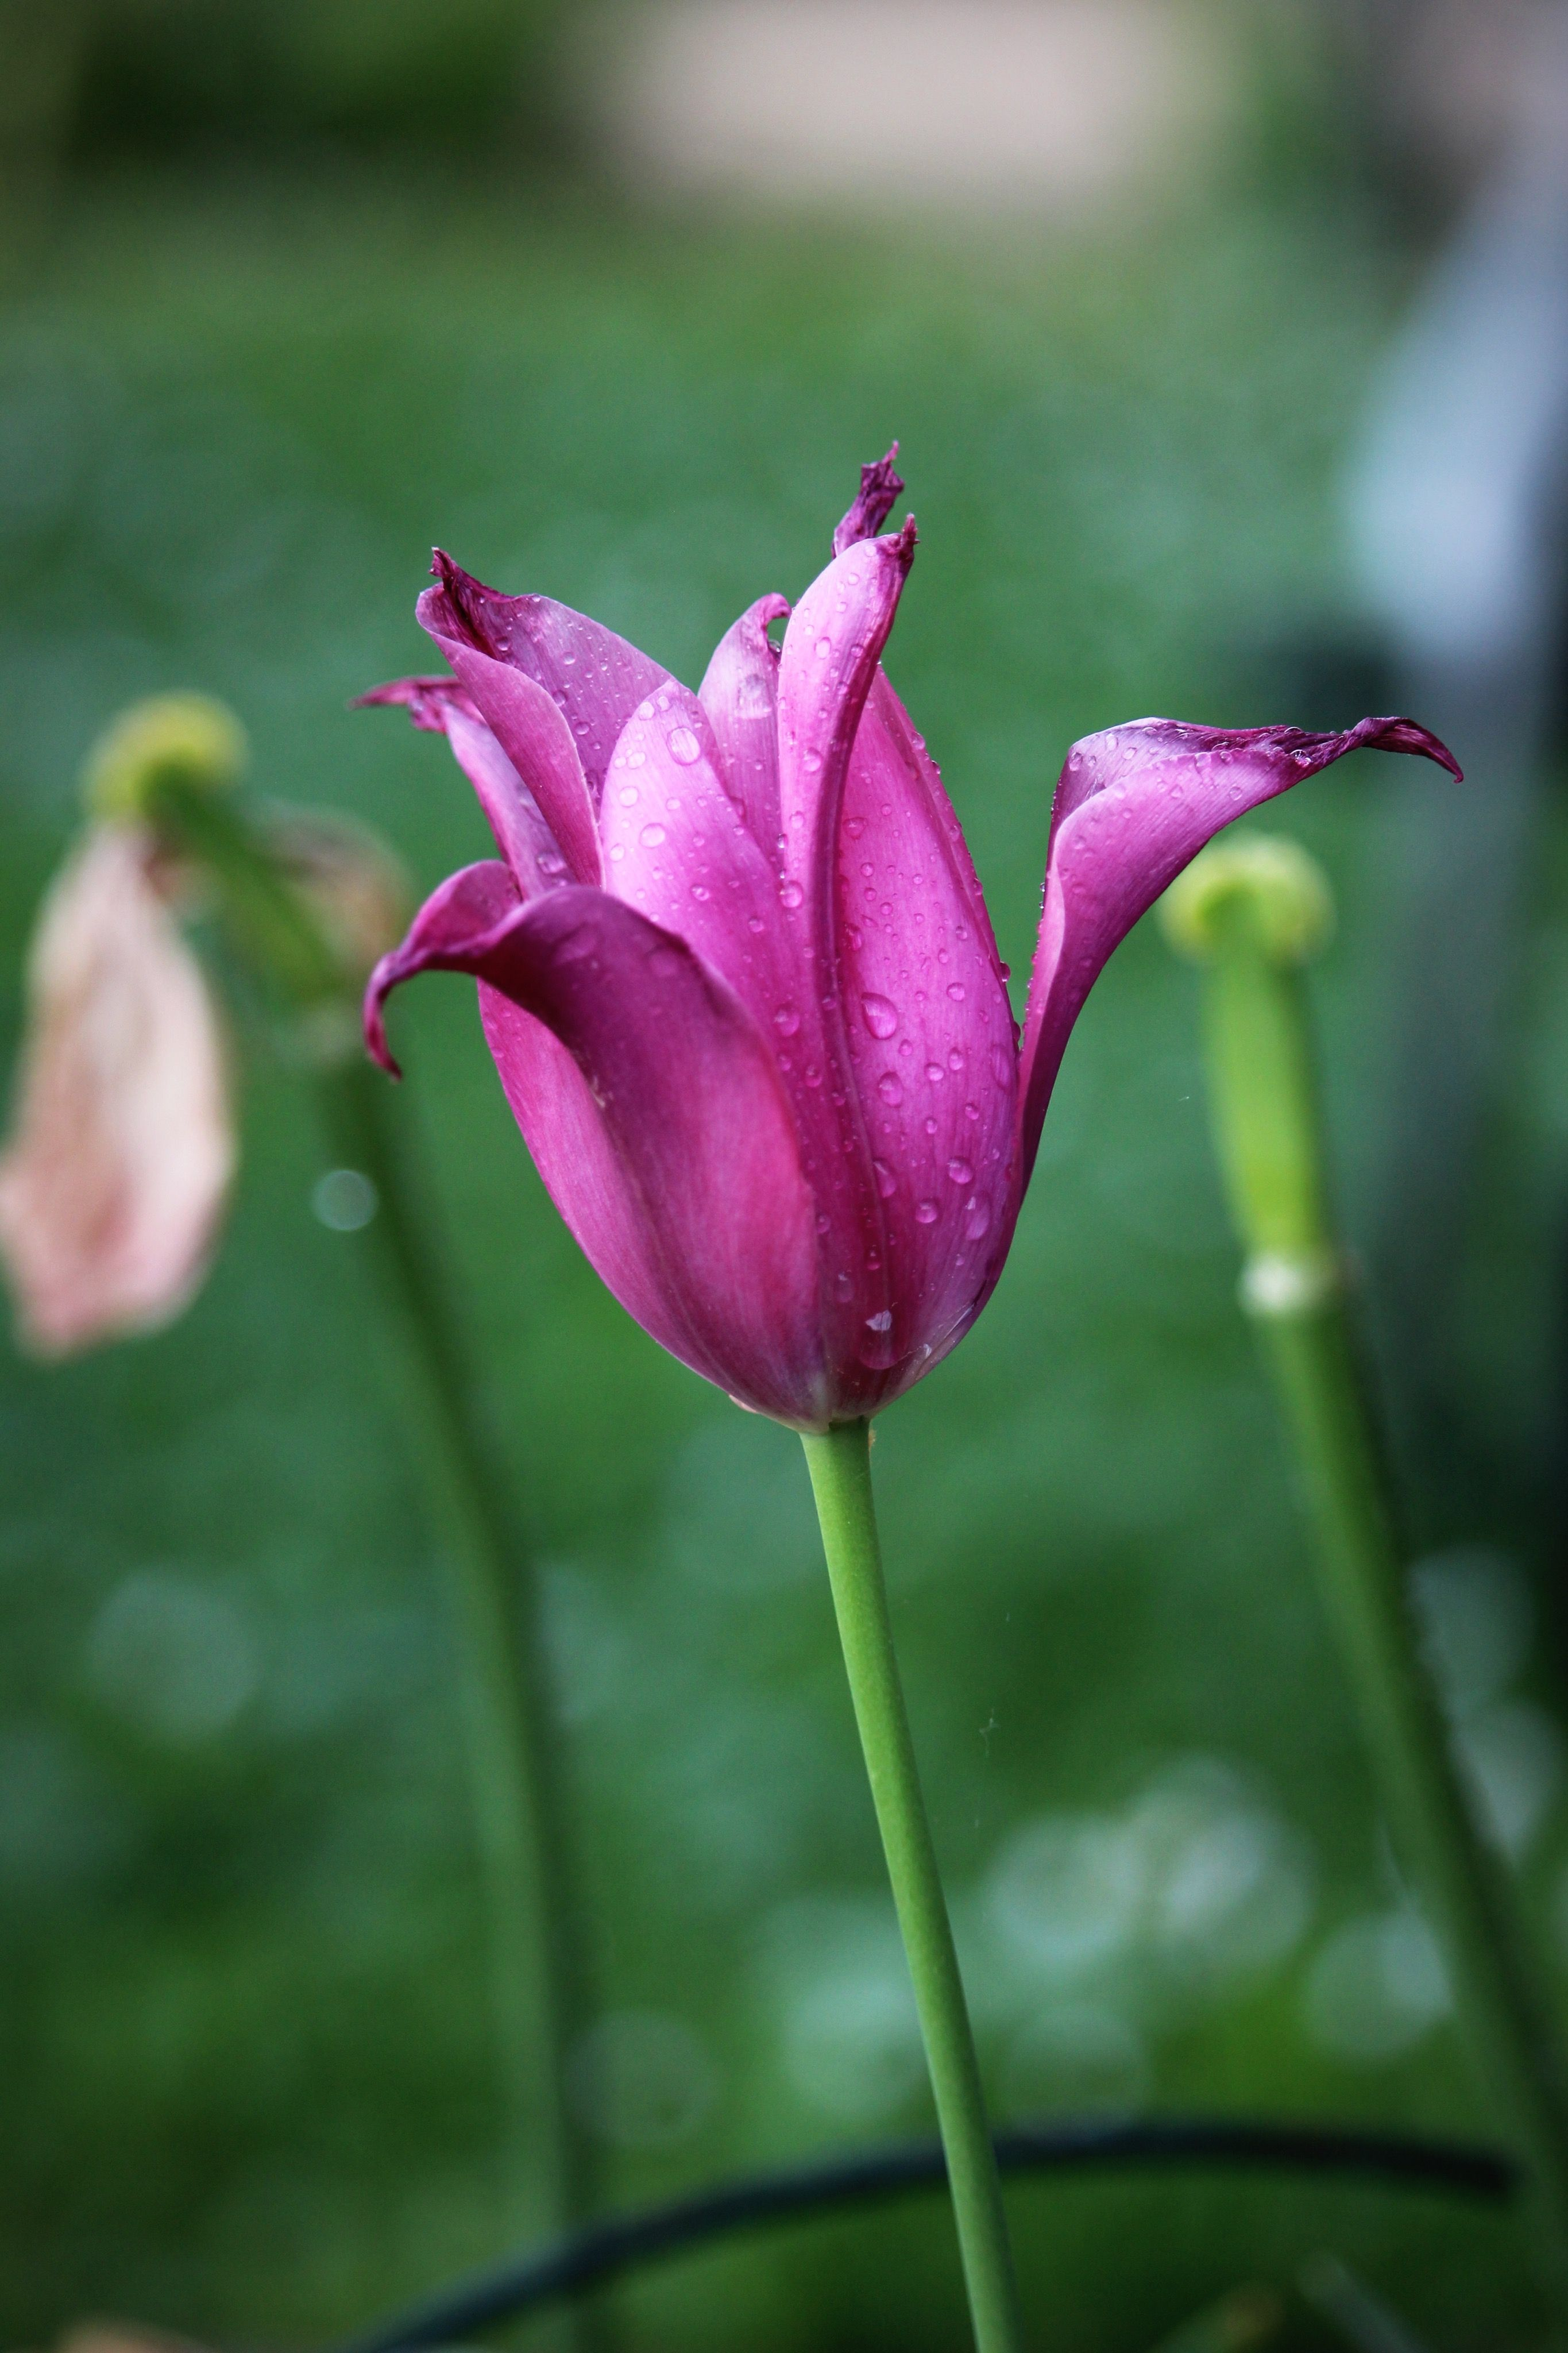
\includegraphics[scale=0.03 ]
		{figures/flower.jpg}}
	\caption{The caption of my figure}\label{fig:flower}
\end{figure}




\section{\textbf{Evaluation}}
\subsection{\textbf{Results}}
The experimental result goes here ... \footnote{https://www.usi.ch}. \\







\newpage
\section{\textbf{Future work}}

\section{\textbf{Summary}}
Future works goes here.






\newpage

%%%%% BIBLIOGRAPHY %%%%%
\bibliographystyle{abbrv}
\bibliography{references}

\end{document}
